\documentclass[10pt,oneside,a4paper]{article}
\usepackage{amsmath}
\usepackage{amsfonts}
\usepackage{amssymb}
\usepackage{fancyhdr}
\usepackage[bottom=0.5in]{geometry}
\usepackage{graphicx}
\usepackage{float}
\usepackage{hyperref}
\usepackage{xcolor}
\usepackage{wrapfig}
\pagestyle{fancy}
\topmargin -0.5in
\lhead{BioE Methods Lab}
\chead{Myoelectric Tetris}
\rhead{Bioelectric Signals}
\begin{document}
\section{Myoelectric Control}
Researchers are currently working on ways to control devices using bioelectric signals. In this portion of the lab you will build an EMG signal classifier to implement myoelectric, or muscle, control in a game of Tetris in Matlab. \\
Goals for week 2:
\begin{enumerate}
\item Myoelectric Control
\begin{enumerate}
\item Learn how to condition and calibrate the EMG signal to create a signal that can be used to control movement of the device
\item Examine the accuracy and precision characteristics of the control signal
\item Use the statistics of the myoelectric control signal to improve the classifier
\item Use the optimized myoelectric control signals to master Tetris
\end{enumerate}
\item EOG control (bonus)
\begin{enumerate}
\item Learn how to condition and calibrate the EOG signal for controlling a computer system
\item Master EOG control to play Tetris!
\end{enumerate}
\end{enumerate}
The procedures for each section are described below. Instructions specific to your report are in \textit{italics font}.
\section{Condition EMG Data, Accuracy and Precision}
Equipment and Supplies: \\
\begin{itemize}
\item Tetris game and controller code available \href{https://github.com/mfliu/Myoelectric_Tetris} {\color{blue} here}. 
\item Vermed Electrodes ($n=5$)
\item SpikerBox and host PC
\end{itemize}
Procedure:
\begin{enumerate}
\item Connect the EMG electrodes to antagonist muscles: biceps vs. triceps, or FCU vs. ECR, etc. Determine which muscles you want to use for left vs. right motion and connect left to Channel 1 and right to Channel 2. Several processing steps are required to convert the raw EMG (i.e. myoelectric) signal into a usable motion command. In the first step, we will ``condition'' the EMG signal by filtering, rectifying, and smoothing the raw EMG. Filtering removes contaminants, such as the motion artifact, and is done with a bandpass filter as studied in week 1 of this lab. The filtered signals are then rectified by taking the absolute value of the filtered signal and smoothing it with a lowpass filter. For these experiments, you will use a cutoff frequency of 2Hz, a fairly low value that produces considerable smoothing of the signal. A higher cutoff frequency could be chosen if you desire a faster time response at the risk of introducing greater variability in the control signal. 
\item Once the raw signals are ``conditioned'', we must determine the usable range of EMG signal that is available, since the maximum amplitude will vary with each muscle, depending on the size of the muscle, the impedance of the muscle, gain of the amplifier, and other things. We can determine the maximum value for each muscle by generating so-called ``maximum voluntary contractions'' or MVCs. Once the EMG amplitude associated with the MVC is determined, we can scale all subsequent EMG measurements for a particular muscle group by this MVC value. This procedure is commonly referred to as ``normalization''. The amplitude range for the ``normalized'' EMG values is between 0 and 1. Run the function \texttt{findMVC.m}. This determines the MVC amplitude for each muscle. Figure 1 shows an example of MVC data that was collected for 4 different muscles. The muscles are labeled according to their ``motion assignments''. These are the directions in which each muscle will be responsible for controlling. For example, we might use the FCU EMG to control ``LEFT'' movements and ECR to control ``RIGHT'' movements. The peak EMG values are noted in each plot, and these can be saved in a data file for retrieval during subsequent operations.  Find and note the MVC values for each desired muscle.
\begin{figure}[H]
\centering
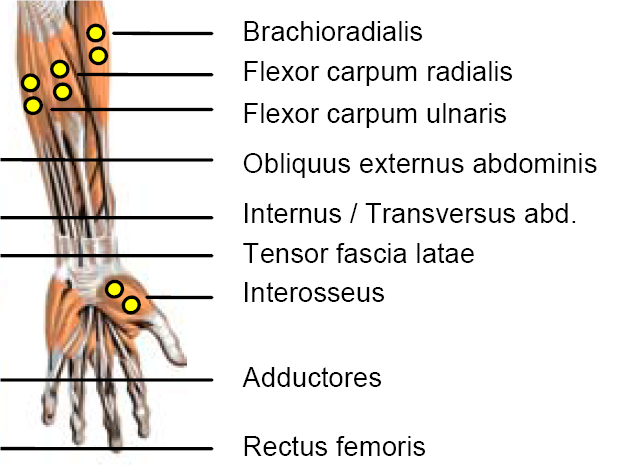
\includegraphics[scale=1]{muscles.png}
\caption{Position of muscles in the forearm. ED is shown in red, ECR in yellow, PL in green and FCU in purple.}
\end{figure}
\begin{figure}[H]
\centering
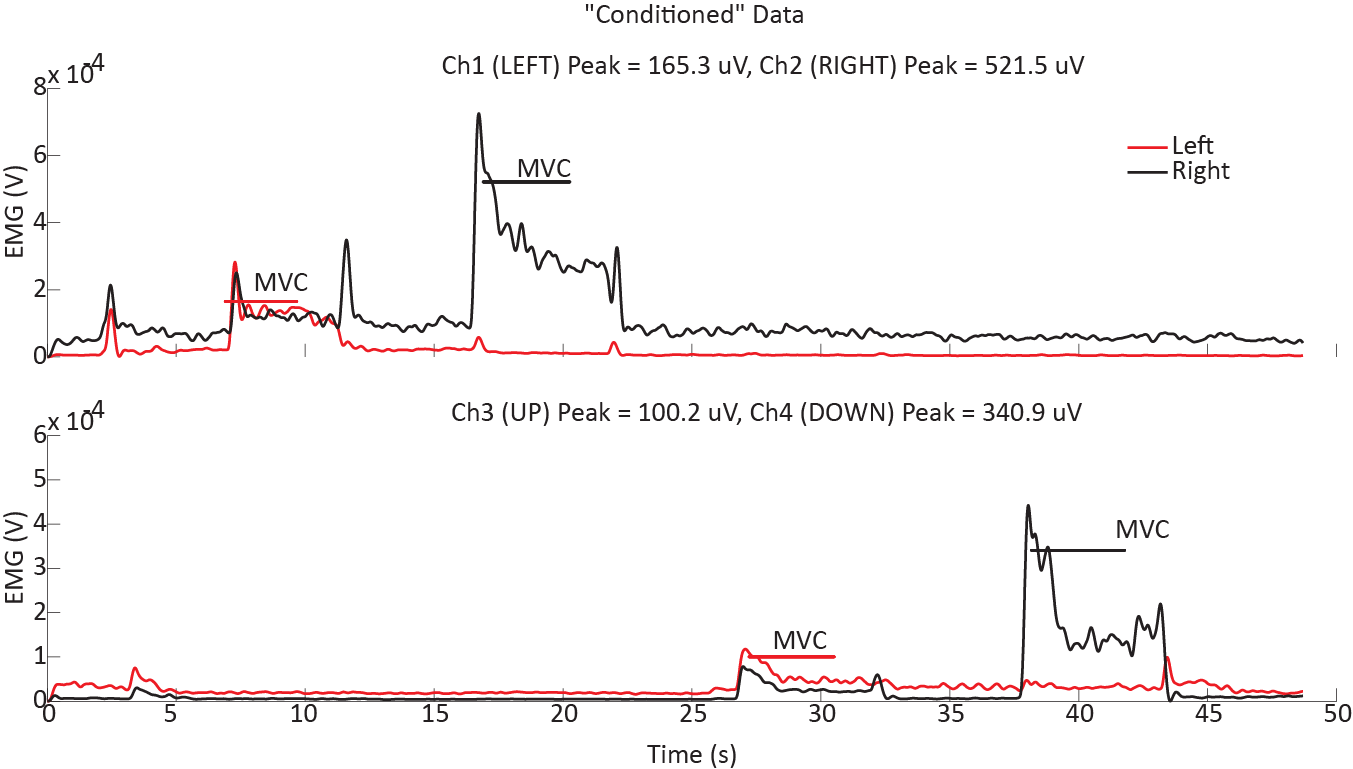
\includegraphics[width=\textwidth]{ConditionedData.png}
\caption{Rectified EMG with MVC indicated for each pair set.}
\end{figure}
\item Once the MVC values for each muscle are determined, we can normalize the subsequent recordings by the MVC. We are now ready to test the myoelectric control performance for each muscle. In the first experiment, we will test the ``Accuracy'' and ``Precision'' of control over a range of contraction levels: 10, 20, 30, 40, 50, and 60\% of MVC.  Run \texttt{StepTrace.m} and follow the traces, controlling your EMG output accordingly.  Track your signal output using SpikeRecorder and record each set.  Figure 3 shows an example of the myoelectric control signals for 4 muscles during step-tracking of these 6 intensity levels or ``setpoints''. The green traces indicate the setpoint levels and the blue traces indicate the normalized (and conditioned) EMG signals.  Use \texttt{MuscleStep.m} for a quick and dirty plot of this process.  Note that some muscles are able to track the setpoint very closely, while others are not as good. In particular, note the ``DOWN'' muscle falls short of reaching the higher setpoints (e.g. 40--60\%). 
\end{enumerate}
\begin{figure}[H]
\centering
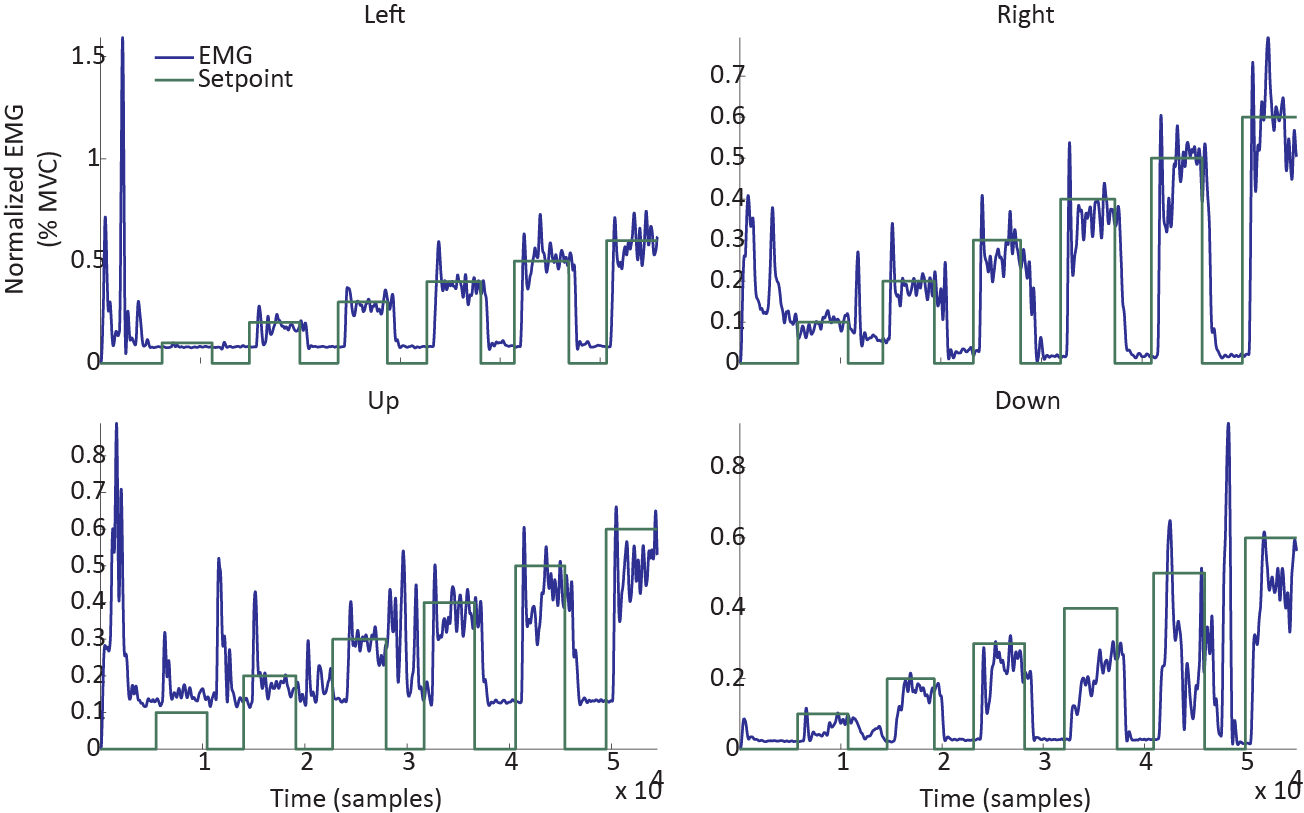
\includegraphics[width=\textwidth]{fig3.png}
\caption{Modulating control via Step-tracking of EMG output}
\end{figure}
We can use this data to quantify the Accuracy and Precision of the myoelectric control signals for each muscle. The Accuracy is defined as the difference or error between the actual myoelectric signal and the target or setpoint as shown in equation 1.
\begin{align}
\texttt{Percent Error} = \frac{\texttt{mean}(M)-T}{T} * 100\%
\end{align}
Where M is the myoelectric control signal (i.e. the normalized, conditioned EMG signal) and T is the setpoint. The precision, which is a measure of the repeatability or reliability of the control signal can be measured at each setpoint as well. We will use equation 2 to do this:
\begin{align}
\texttt{Percent Deviation} = \frac{\texttt{std}(M-T)}{T} * 100\%
\end{align}
\textit{In your write-up, discuss the trends that you observe in the accuracy and precision of the myoelectric control signal across the range of intensity levels that were tested. Figure 4 shows an example of the Accuracy and Precision characteristics for the myoelectric control signals shown in Figure 3. As you may have also noted in Figure 2, on most channels, the error and deviation tend to change with the setpoint level. Also note the polarity of the error--is it positive or negative? What does the polarity indicate? What does the deviation indicate? Think about the effects that the error and deviation may have on control performance. Are the trends important? In other words, does it matter that the accuracy and precision change with myoelectric signal intensity? Finally, discuss how this information could be used to tune the performance of your myoelectric controller.}
\begin{figure}[H]
\centering
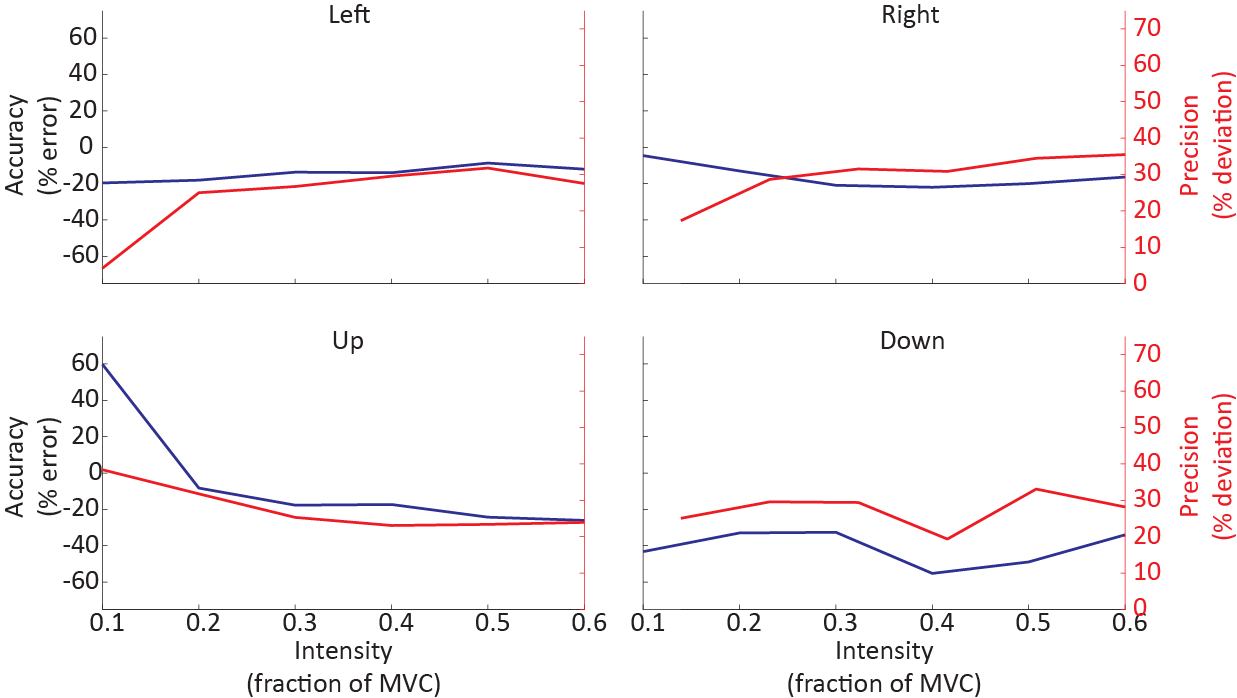
\includegraphics[width=\textwidth]{fig4.png}
\caption{Example of accuracy and precision characteristics}
\end{figure}
\section{Myoelectric Tetris Setup}
Startup the ``Myoelectric Tetris'' module (see link above).  Follow the setup instructions to start interacting with the game.  This game classifies the overall muscle activity into three states to allow for leftwards, rightwards, and block rotation control.  You will use the two antagonistic pairs like the ones you trained with before.  You will be adjusting the RMS values (see below), the window size, and the gain functions (percent MVC or normalized EMG values) to tune your control signals.  \textbf{Note:} this is not continuous velocity-based control.  Keep in mind what the differences would be\dots
\subsection{Software Setup}
Streaming data from SpikerBox into Matlab requires a separate USB interfacing library that is implemented in Python. To get data in real time from SpikerBox, you will need to install Python and the Python USB library \texttt{hidapi}. The next several sections take you through how to install Python and the \texttt{hidapi} library.
\subsubsection{Installation on Windows}
Matlab Tetris requires Python to be installed to interface with the USB. This section walks through how to install Python, \texttt{pip}, and \texttt{hidapi}. If you already have any of these installed, jump to the appropriate section.
\subsubsection{Install Python}
To install Python, download the \href{https://www.python.org/ftp/python/3.6.4/python-3.6.4-amd64.exe}{\color{blue}Python installer} from Windows if you have a 64-bit computer. On the first screen, make sure to check the box that reads ``Add Python 3.6 to PATH''. Select ``Install Now'' and click ``Yes'' if your computer asks for administrator privileges: 
\begin{figure}[H]

\includegraphics[width=\textwidth]{image.png}
\end{figure}
Once installation has completed, open ``Command Prompt'' in your start menu and ensure that Python is installed by typing \texttt{python} into the command line and pressing enter. If you see ``Python 3.6.4'' and other details, then Python has been correctly installed:
\begin{figure}[H]
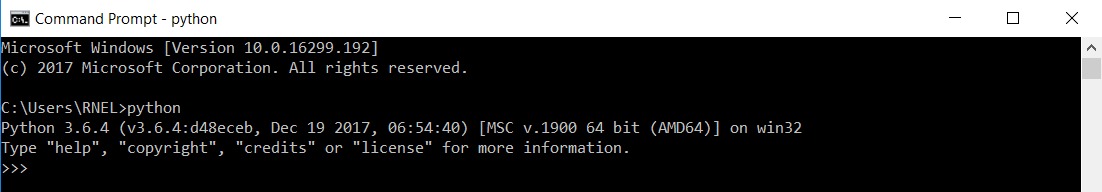
\includegraphics[width=\textwidth]{commandline.png}
\end{figure}
\subsubsection{Install \texttt{pip}}
Install \texttt{pip} by downloading the \href{https://bootstrap.pypa.io/get-pip.py}{\color{blue}script} \textbf{into your user directory} \texttt{(C:\textbackslash Users\textbackslash <USER>)}. Exit the Python shell in the command line by typing \texttt{exit()} and install \texttt{pip} with the command:
\begin{verbatim}
python get-pip.py
\end{verbatim}
\begin{figure}[H]
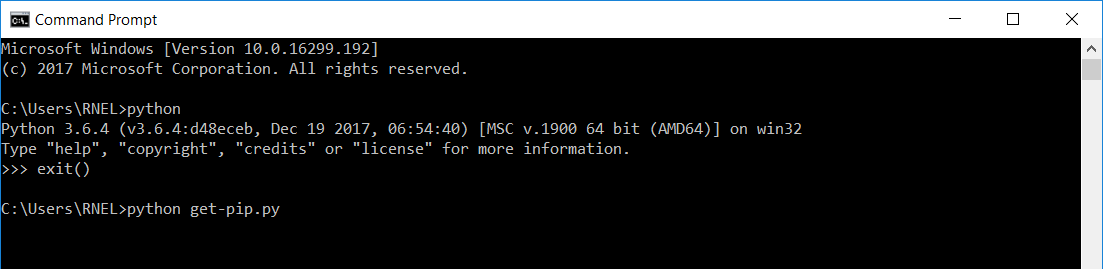
\includegraphics[width=\textwidth]{pip.png}
\end{figure}
Verify that \texttt{pip} is installed by typing \texttt{pip -version} into the command line and pressing \texttt{Enter}:
\begin{verbatim}
C:\Users\RNEL>pip --version
\end{verbatim}
You should see a similar output:
\begin{verbatim}
pip 9.0.1 from c:\users\rnel\appdata\local\programs\python\python36\lib\site-packages
\end{verbatim}
This means that \texttt{pip} has been successfully installed.
\subsubsection{Install \texttt{hidapi}}
The easiest way to install \texttt{hidapi} is through \texttt{pip} on Windows. In the command prompt, install  \texttt{hidapi} with the following command and press enter:
\begin{verbatim}
C:\Users\RNEL>pip install hidapi
\end{verbatim}
A quick (optional) way to test your \texttt{hidapi} install is to run the following commands:
\begin{verbatim}
C:\Users\RNEL>python
\end{verbatim}
Then, in the Python shell, try:
\begin{verbatim}
>>> import hid
\end{verbatim}
If the import succeeds, \texttt{hidapi} has been successfully installed.
\subsection{Download Myoelectric Tetris}
Download the code for \href{https://github.com/mfliu/Myoelectric_Tetris} {\color{blue} Myoelectric Tetris} by downloading the \texttt{.zip} file and unzipping it into a directory of your choice. In the directory, there should be the following files: \\
\begin{enumerate}
\item \texttt{emg\_buffer.py}: This is the Python script that gets EMG data from SpikerBox. \textbf{Do not change this file}.
\item \texttt{py\_emg\_buffer.m}: The Matlab connector to \texttt{emg\_buffer.py}. \textbf{Do not change this file either.}
\item \texttt{test\_emg\_buffer.py}: A simple Python script to test the USB interface manager implemented in \texttt{emg\_buffer.py}. Running this in a Python shell allows for debugging of the Python USB library, but should not be necessary for this portion of the lab.
\item \texttt{matlabtetris.m}: The main function that runs Tetris in Matlab, reads EMG data from SpikerBox, and calls the EMG classification function that you write. Run this function to start a game of Tetris.
\item \texttt{set\_window\_size.m}: Set the time window of EMG to buffer for classification, in milliseconds. 
\item \texttt{emg\_control.m}: The EMG signal classifier. This Matlab script takes in two channels of raw EMG input and outputs an array of length 3 corresponding to the direction the Tetris piece should move (left, right, or turn).
\end{enumerate}
\section{Implementing Myoelectric Control}
In this portion of the lab, you will be adjusting settings on a root-mean-square-based EMG classifier to control pieces in a game of Tetris. Hook up the SpikerBox to electrodes on wrist flexor-extensor muscle pair on your left forearm and turn SpikerBox on. Try running \texttt{matlabtetris.m}. You should see the Tetris game pop up in a new window. Press \texttt{Start}. The game should begin, and you will see a scatter plot of RMS values from each EMG channel. Flexing your wrist will move the Tetris piece to the left, extending your wrist will move the piece to the right, and co-contracting flexors and extensors will cause the Tetris piece to rotate counterclockwise. 
\begin{enumerate}
\item Once the game is running in matlab, you will first attempt to make stereotyped motions to establish how well the classifier is functioning.  For one muscle, record 10 stereotyped motions while running the game.  Continue with the opposing muscle.  Finish by attempting co-contracting motions.  The system measures EMG data with a particular window size (default is 100 ms).  
\item Use the \texttt{plot\_RMS.m} function to plot your stereotyped behaviors. Fit each muscle set and adjust your RMS thresholds in \texttt{emg\_control.m} appropriately.  Also adjust gains as per the previous MVC calibration steps.  You can also play with \texttt{set\_window\_size.m} to make the system more sensitive.  At each change step, track your classification parameters as a function of game performance.  Provide a rationale with the data you collect to explain the tuning decisions you make.
\begin{figure}[H]
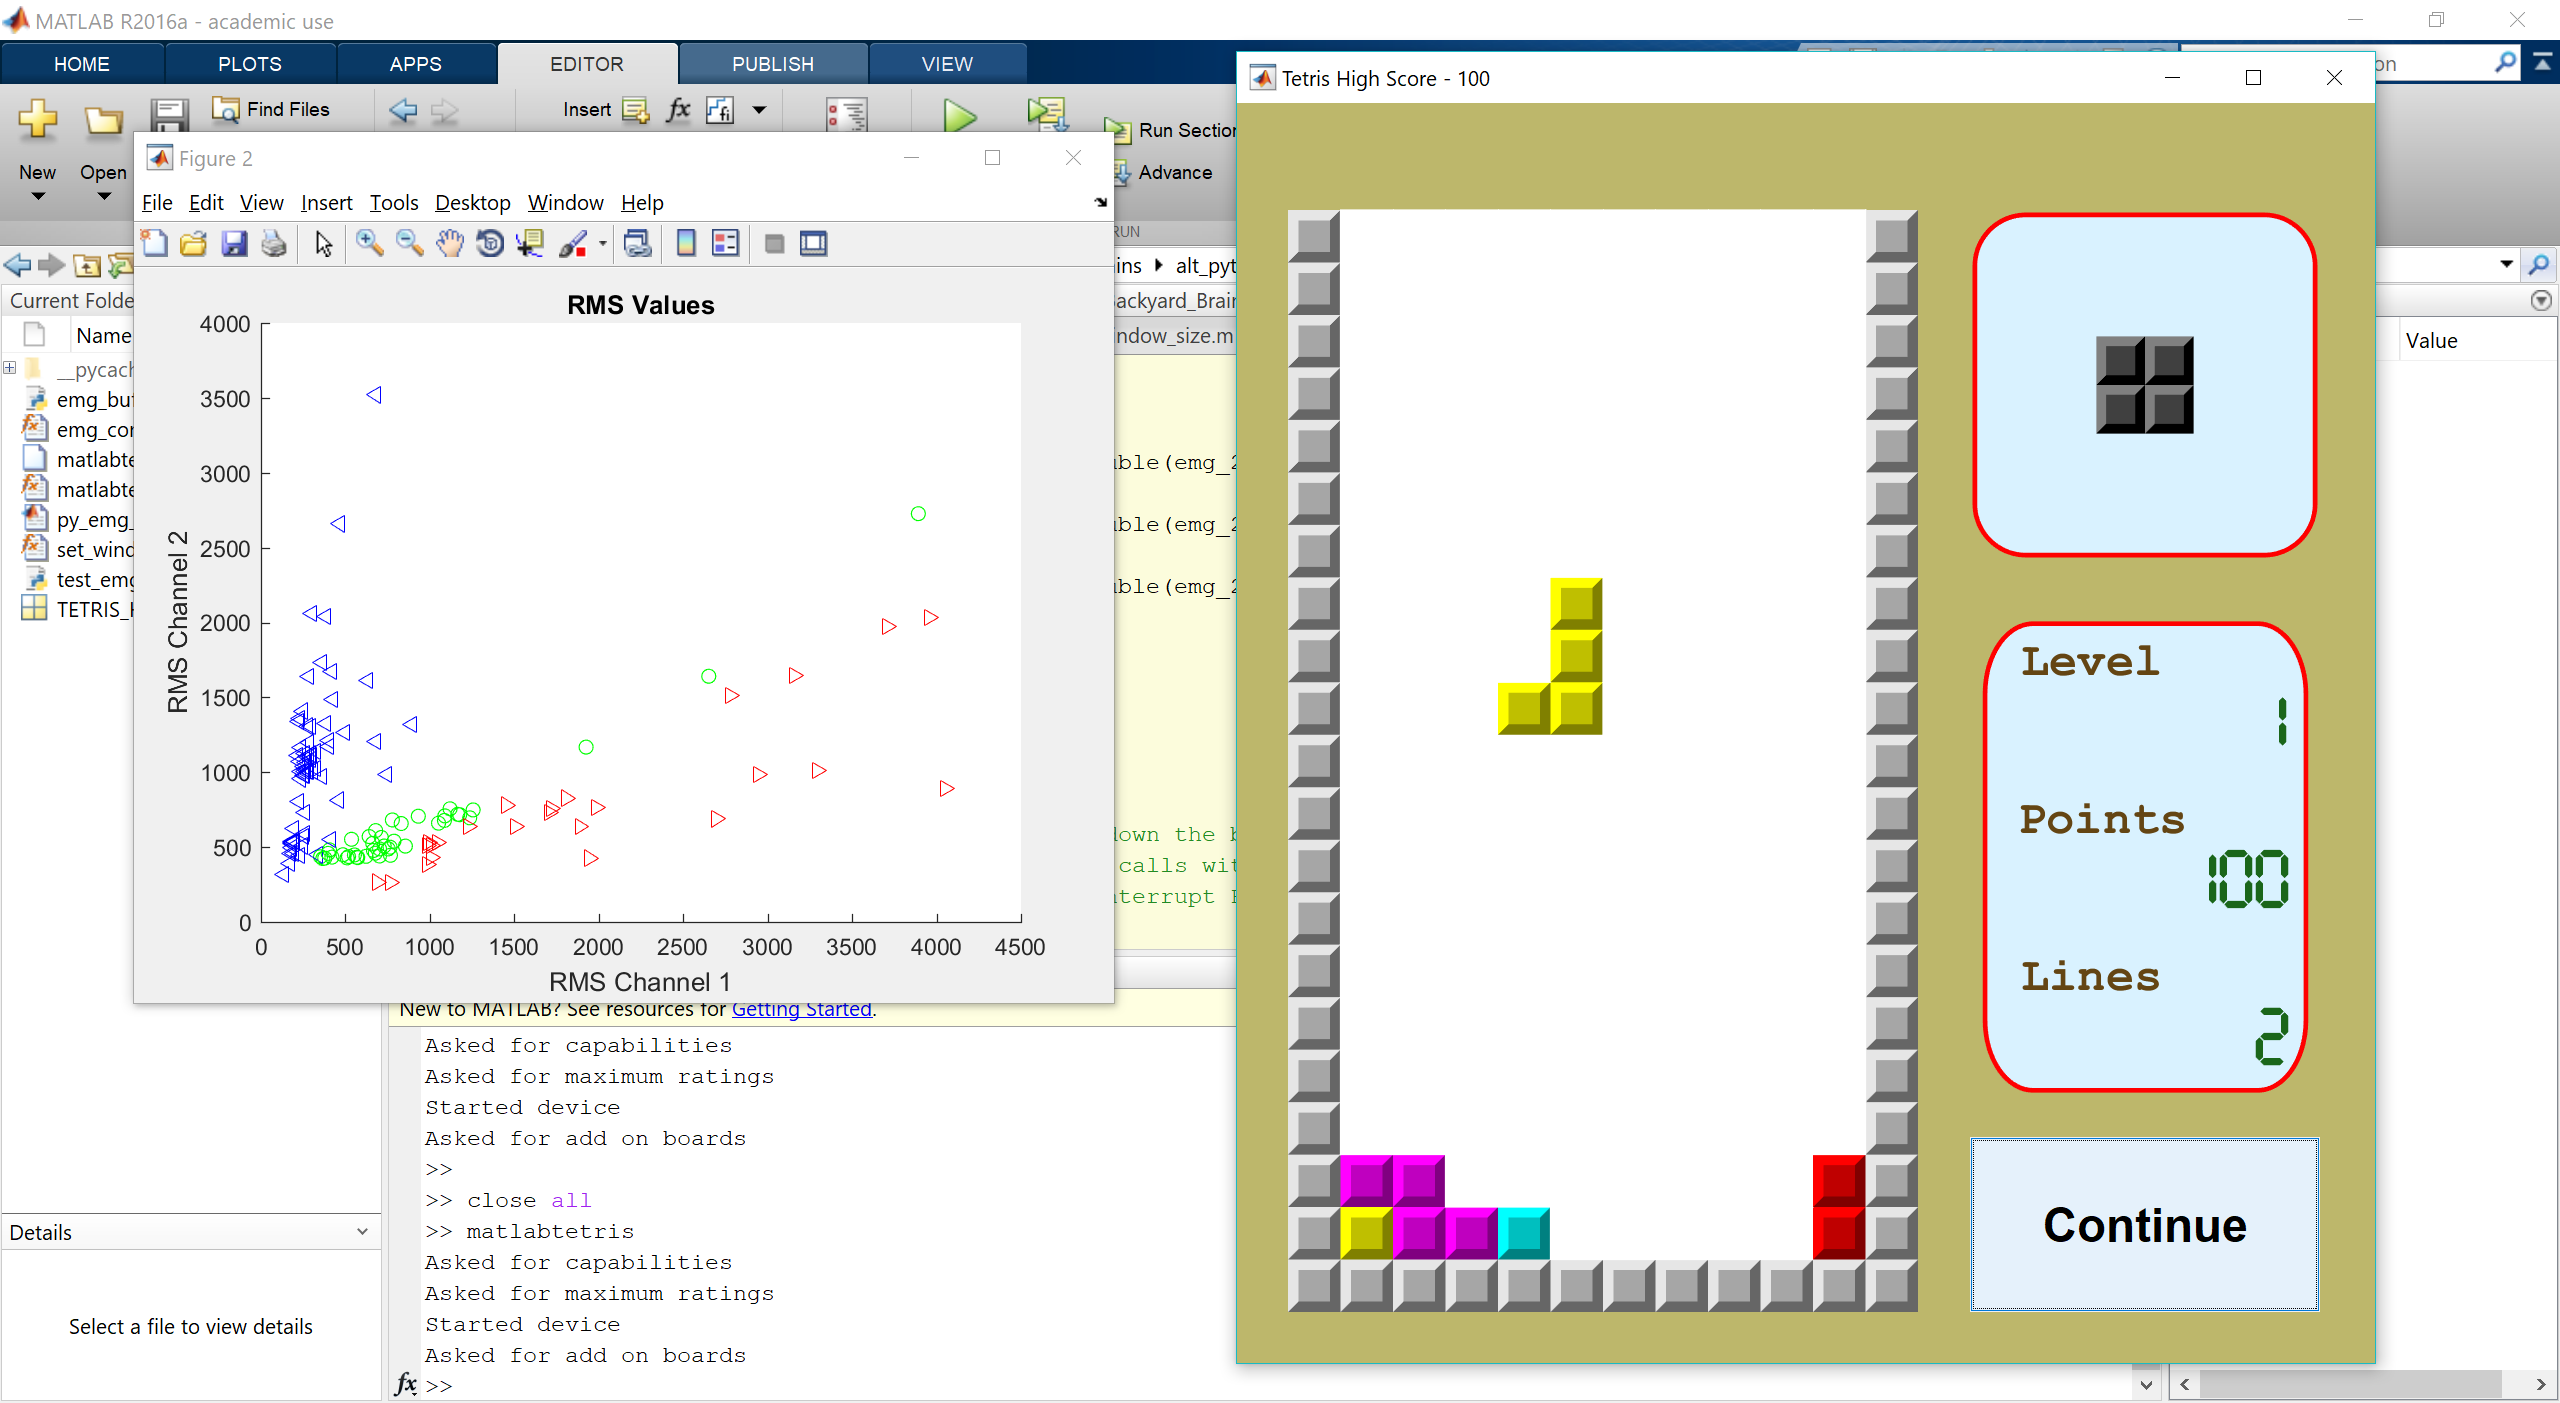
\includegraphics[width=\textwidth]{tetris_game.PNG}
\end{figure}
\item The classifier you build will take a snippet of raw EMG signal from the two muscles and determine if the movement giving rise to that signal was a wrist flexion (move Tetris piece right), wrist extension (move Tetris piece left), or co-contraction (rotate Tetris piece clockwise). It performs this classification at each time step and updates the position of the Tetris piece according to the output of the classifier. In a single timestep, a Tetris piece \textit{must} make one movement downward and \textit{may} make one movement out of \{move left, move right, rotate\}.
\item Try to get the highest score!  Compare your optimized results with your fellow groups.  Also, compare how modulation control compares to game performance.  How did that initial training help?  What else could you adjust to improve game performance?
\end{enumerate}
\textit{In your write-up, discuss the quality of the control performance that you were able to achieve. Was it easier to control leftwards motion than rightwards motion or vice-versa? Was the classification for one direction better than the other? What was the effect of co-contraction? How might this affect the performance? Is the object control fast or slow? Was the control intuitive or did it require a lot of intense concentration? Finally, discuss the usefulness of this approach for controlling a prosthesis or other virtual system. If you needed to use a prosthesis, would you want myoelectric control? Discuss ways that the control might be improved – focus on the problems (e.g. speed, accuracy, reliability) – and propose some solutions. Would you want to use different signal processing methods, more control channels, etc\dots ?}

\subsection{RMS Classification}
Open \texttt{emg\_control.m}. This Matlab function is where the classifier is implemented. It takes as input the raw signal of two EMG recording channels, which provide signal from your wrist flexor muscle and wrist extensor muscle. Using these raw EMG signals, \texttt{emg\_control.m} computes the RMS of the signal on each channel and performs a simple thresholding based on the ratio of the RMS of the two channels. The function returns an array of length 3, where a value of 1 in the first element means the Tetris piece should move left (extension), a value of 1 in the second element means the piece should move to the right (flexion), and a value of 1 in the last element indicates the Tetris piece should turn in the clockwise direction (co-contraction). Since you can only perform one movement per time step and the Tetris piece can only make one movement per timestep, only one element in the vector is nonzero for a single EMG snippet. This is called a \textbf{one-hot encoding} scheme. 
\begin{verbatim}
function [left, right, turn] = emg_control(emg_1, emg_2)
left = 0;
right = 0;
turn = 0;

rms_1 = rms(emg_1);
rms_2 = rms(emg_2);
\end{verbatim}
 
Currently, the classifier is a rough threshold on the ratio of RMS of channel 1 to RMS of channel 2. Think about how you should set the thresholds on the RMS ratio based on which muscles your electrodes are hooked up to. For example, if channel 1 is recording the wrist flexors in your forearm, then a RMS ratio $\frac{RMS(Channel1)}{RMS(Channel2)} > 1$ would indicate that the wrist flexor muscles are contracting more strongly than the extensor muscles, so the piece should move to the left. Similarly, if the RMS ratio $\frac{RMS(Channel1}{RMS(Channel2)} = 1$, then your flexors and extensors are co-contracting approximately equally, which would mean you should turn your Tetris piece. 
\begin{verbatim}
if rms_1/rms_2 > 1.8
    right = 1;
elseif rms_1/rms_2 < 0.8
    left = 1;
elseif rms_1/rms_2 > 0.8 && rms_1/rms_2 < 1.8
    turn = 1;
end
\end{verbatim}
Think about what thresholds or aspects of the EMG signal you would want to use for classification. The scatter plot of RMS values of each channel may help you.

The scatter plot in the figure above shows the classification of each point. As you classify EMG signals during the game, a point corresponding to (RMS(Channel1), RMS(Channel2)) will be plotted in the scatter plot with the color and shape indicating what your classifier labeled that point as. {\color{blue} Blue arrows} pointing left indicate that the classifier predicted that the Tetris piece should move left, {\color{red} red arrows} pointing right indicate the Tetris piece moved right, and {\color{green} green circles} indicate that the Tetris piece rotated.

Try playing Tetris a couple times and look at where the RMS values fall. Move the Tetris piece with some flexion, extension, and co-contraction movements. If your electrodes are on your left arm, then a wrist flexion indicates that the Tetris piece should move to the right. Look at where the point shows up--does the classifier indeed plot a red rightward arrow for that point? Try a couple of other movements. Where do these points fall? Are there decision boundaries you can draw in this two-dimensional RMS space that will help you classify the movement the Tetris piece should do? Change the \texttt{if} statements in \texttt{emg\_control.m} to RMS ratios or threshold values that you think will classify the EMG signal the best. 
\subsection{EMG Window Size}
Another factor in classification accuracy is the time window of EMG signal that we use. In \texttt{set\_window\_size.m}, set the length of the EMG signal (in milliseconds) you want to use for classification. Try different values ranging from 5ms to 500ms. What are the advantages of using a shorter time window? A longer time window?
\begin{verbatim}
function window_size = set_window_size()
window_size = 100; % in ms
end
\end{verbatim}
\section{EOG and its use for Computer Cursor Control}
With a different biological signal there are new control concerns and approaches to try and control some device. In this case we will be using EOG to control the position of a computer cursor.  As is necessary when using a biological signal we will first seek to understand some of its basic properties. \\
\begin{wrapfigure}[4]{r}{0.4\textwidth}
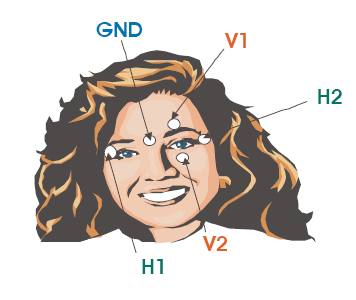
\includegraphics[width=0.3\textwidth]{eog.png}
\end{wrapfigure}
Equipment and Supplies: \\
\begin{itemize}
\item Vermed Electrodes ($n=5$)
\item Bioradio and host PC
\item Measuring tape
\end{itemize}
Procedure:
\begin{enumerate}
\item Place the electrodes as shown to the right.  We will be using the ground, the horizontal electrodes (H1 and H2), and the vertical electrodes (V1 and V2).
\item With the electrodes in place examine the general characteristics of the signal, and the following situations:
\begin{enumerate}
\item DC relation to head angle
\item Head movement
\item Blinking
\item Drift
\item Light
\end{enumerate}
\item Center your eyes at a comfortable distance back from the screen and run through classification as before.  Set the gain and RMS values to allow for 3 sources of control as you see fit.  Be prepared to discuss why these parameters.
\item Instead of setting the gain as a function of MVC, recalibrate with your head closer to the screen (about 40cm) and retry using this determined relationship to play Tetris.  Did this make a significant difference in control?
\end{enumerate}
\textit{In your write-up, discuss the challenges associated with calibrating and using the EOG signal for object control. Discuss the similarities and differences between EOG and EMG in relation to signal conditioning. Was the EOG control reliable throughout the entire period of use? Why or why not? Is frequent recalibration necessary? Compare your EOG control and myoelectric control experiences? Discuss situations where one approach may be more appropriate than the other.}
\section{General Topics for Discussion}
\begin{enumerate}
\item Importance of and procedures for signal conditioning
\item Accuracy and Precision of control with bioelectric signals
\item Human factors issues with these approaches for device control: Aesthetics, portability, user-friendliness--compare to other alternatives for prosthetic arm and computer control in persons with disability
\end{enumerate}
\end{document}